%%================================================
%% Filename: chap04.tex
%% Encoding: UTF-8
%% Author: Yuan Xiaoshuai - yxshuai@gmail.com
%% Created: 2012-04-28 00:15
%% Last modified: 2019-11-06 17:39
%%================================================
\chapter{基于多模态特征融合的 ResNet-BiGRU 分类检测模型}
\label{cha:ResNet-BiGRU}
% 在当今的网络环境中,流量数据的海量性和高维性已成为其显著特点,这不仅为网络威胁检测带来了前所未有的挑战,也为数据分析和安全预防提出了更高要求。
% 传统检测方法虽然在某些场景下取得了不错的成绩,但通常侧重于单一维度的分析,如基于规则的检测或基于特定特征的分类,往往未能充分发掘流量数据中蕴含的空间特征和时序特征。
% 这种方法在处理静态或简单模式的威胁时可能足够,但面对复杂的攻击手段,尤其是持续演化的网络威胁,其检测效率和准确性显然有很大的提升空间。
% 此外,随着网络技术的快速发展和应用的日益广泛,网络攻击手段也变得更加多样和隐蔽,常常涉及复杂的行为模式和多步骤的攻击策略,这便要求威胁检测系统能够理解和分析数据的深层特征及其在时间序列上的演变规律。
% 然而,传统方法在这方面的能力较弱,难以有效捕捉到这种复杂性,特别是在对加密流量或未知新型攻击的检测上,更是力不从心。\par

% 针对传统网络攻击检测方法不能综合考虑流量数据中蕴含的空间特征和时序特征,且检测效率和准确性仍有很大的提升空间的问题,本文设计并提出了一种多模态特征融合的ResNet-BiGRU模型,旨在综合利用深度学习中的残差网络(ResNet)和双向门控循环单元(BiGRU)的优势,以更全面地挖掘网络流量数据中的空间和时序特征。
% 该模型利用先进的多模态特征融合技术,综合模型提取的空间特征和时序特征进行分析决策,大大提高了对复杂攻击模式的识别能力。
由于传统网络攻击检测方法不能综合分析流量数据中的空间特征与时序特征,网络攻击检测的准确性仍有很大的提升空间。
针对此问题,本文设计并提出了一种基于残差网络(ResNet)与双向门控循环单元(BiGRU)的多模态特征融合模型。
该融合模型充分结合了ResNet在挖掘空间特征方面的优势与BiGRU在捕捉时序特征方面的长处。
通过深度解析流量数据中的空间特征和时序特征,模型实现了两者的综合分析,进而显著提升了攻击检测的准确性。
% 此外,通过对海量高维数据的深度学习处理,该模型还能自动识别和学习最具区分力的特征,进一步提升了检测的准确性和鲁棒性。
% 总的来说,本文的研究不仅指出了传统网络威胁检测方法的局限,也为利用深度学习技术提升网络安全防御能力提供了新的视角和方法。
% 在现代网络安全领域,快速准确地检测潜在攻击的能力至关重要。
% 但是,我们面临的挑战在于,传统的攻击检测方法往往依赖于预先定义的特征集,这可能导致对新型攻击的检测能力不足,因为它们无法适应不断变化的攻击模式。
% 另外,实际的流量数据有着海量高维的特点,然而常规的算法通常不会针对这种特点进行调整适应,往往结果是生成的模型在实际部署中准确率低、误报率高。
% 因此,为了能够解决这种概念漂移问题和能够有效挖掘复杂网络数据的深层特征以达到更高的检测精度,我们引入了基于特征选择优化的 ResNet-BiGRU 分类检测模型。
% 图~\ref{fig:attack_detecion_model}~描述了我们的检测模型的工作原理和流程。
% \begin{figure}[htbp]
%   \centering
%   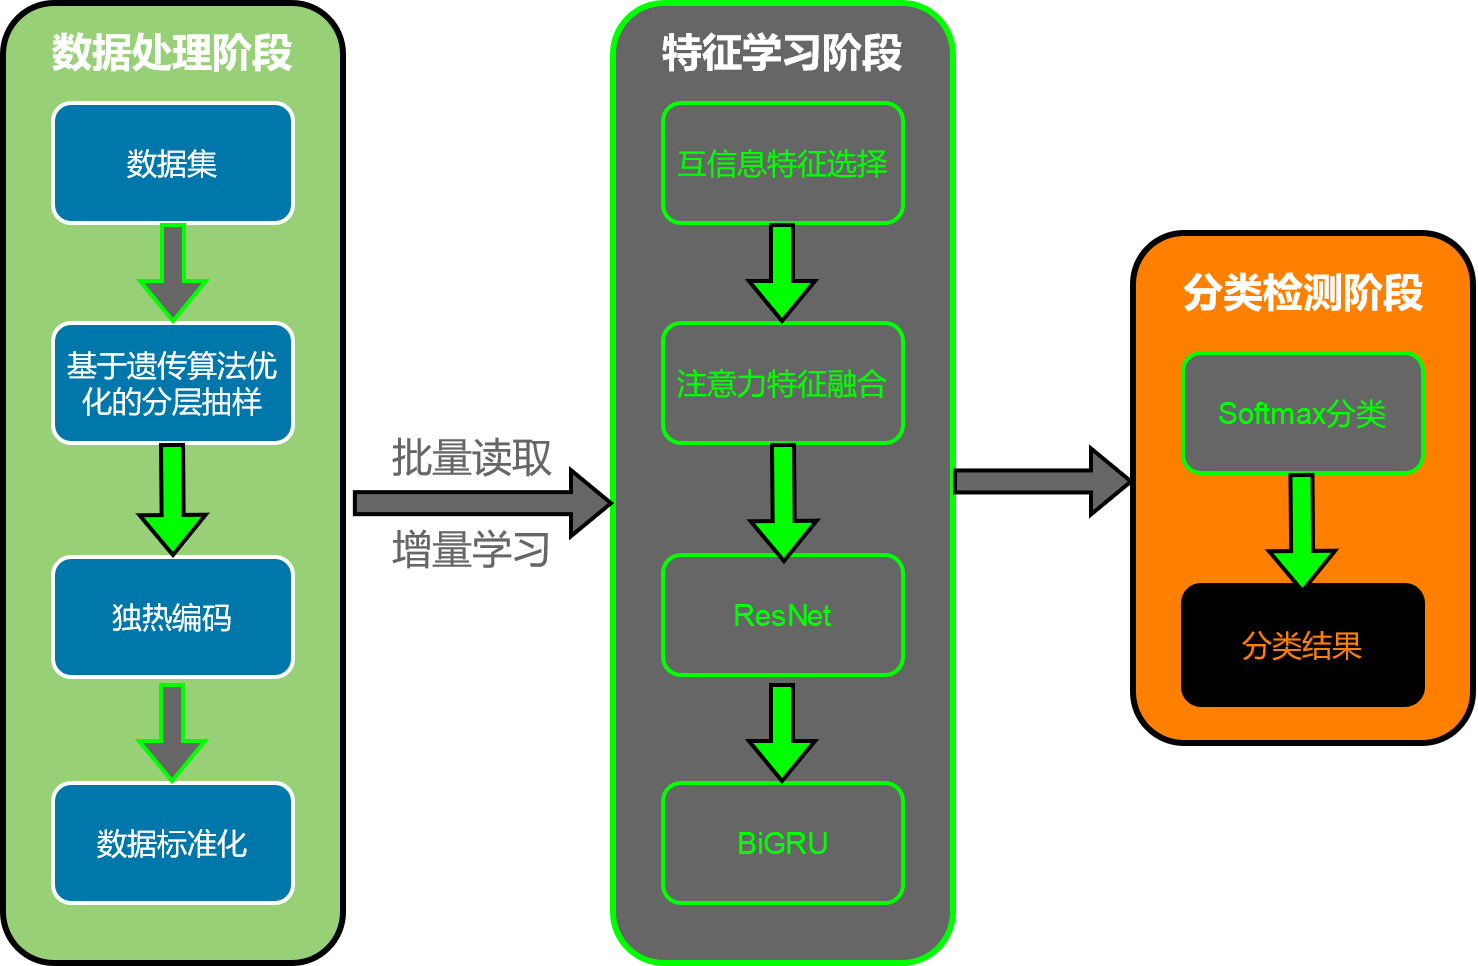
\includegraphics[width = 0.8\textwidth]{ourmodel.drawio.png}
%   \caption{基于特征选择优化的 ResNet-BiGRU 分类检测模型}
%   \label{fig:attack_detecion_model}
% \end{figure}


% 模型首先采用遗传算法对分层抽样过程进行优化,保证训练集的质量;
% 之后利用互信息冗余算法进行特征降维来提高算法效率减少过拟合的风险;
% 训练采用增量学习的方式适应不断变化的攻击模式,减少对数据集的依赖性;
% 最后利用ResNet-BiGRU的优势来解决深度网络中的梯度消失问题、捕捉时间序列数据中的长期依赖关系,从而挖掘复杂网络数据的深层特征,提高检测精度和准确率。
% 接下来,我们将详细地从实验数据集、数据集预处理、模型具体结构设计、实验设置、实验结果逐步展开介绍。

\section{方法概述}
% 网络通信涉及复杂的交互模式,包括客户端与服务器之间的请求响应、数据传输过程中的拥塞控制等。
% 这些交互在空间上体现为数据包的具体内容,如源IP地址、目标IP地址、端口号、协议类型等,这些信息在数据包的特定位置以特定格式存在,形成了数据的“空间”结构。
% 在时间上则表现为交互的顺序和持续时间。\par
该方法主要通过多模态特征融合技术将ResNet以及BiGRU进行融合,从而综合分析网络流量数据中的时空特性,提升决策性能。
该方法的原理在于,首先,ResNet提取网络流量数据中的深层次空间特征,BiGRU则捕捉流量数据时序特征的前后依赖关系。
接着,结合这两个特征形成混合的时空特征。
最后,综合ResNet和BiGRU的决策输出以及混合的时空特征,结合三者,产生产生最终的决策输出。
\subsection{多模态特征融合设计}
多模态特征融合是一种将来自不同来源或类型(模态)的数据集成在一起的过程,目的是改善决策过程、预测准确性或数据解释能力。
这些不同模态的数据可能包括文本、图像、视频、音频和传感器数据等。
在机器学习和深度学习领域,多模态特征融合已成为一个重要的研究领域,尤其是在需要综合处理不同类型数据的应用中,如自然语言处理、计算机视觉、语音识别和人机交互等。
融合策略通常可以分为早期融合、晚期融合、混合融合三种类型。\par

早期融合(如图~\ref{fig:MultimodalFusio} (a)~所示),也称为特征级融合,这种策略在模型的某个中间层面整合不同模态的特征。
早期融合旨在利用深度学习模型的能力来学习和利用不同模态之间的相互作用。\par

在晚期融合(如图~\ref{fig:MultimodalFusio} (b)~所示)策略中,每个模态分别处理并做出决策或预测,最终的融合是在决策或预测级别进行的,例如通过投票、平均或学习到的加权组合。
晚期融合能够保持模态之间的独立性,适用于模态之间关联不强的情况。\par

混合融合(如图~\ref{fig:MultimodalFusio} (c)~所示)策略结合了上述几种融合策略的元素,以期在不同模态的特征提取和决策过程中利用各种融合方法的优点。
例如,一个混合融合框架可能会同时使用早期融合来捕获一些模态之间的直接关系,以及晚期融合来维持某些模态的独立性。

\begin{figure}[htbp]
  \centering
  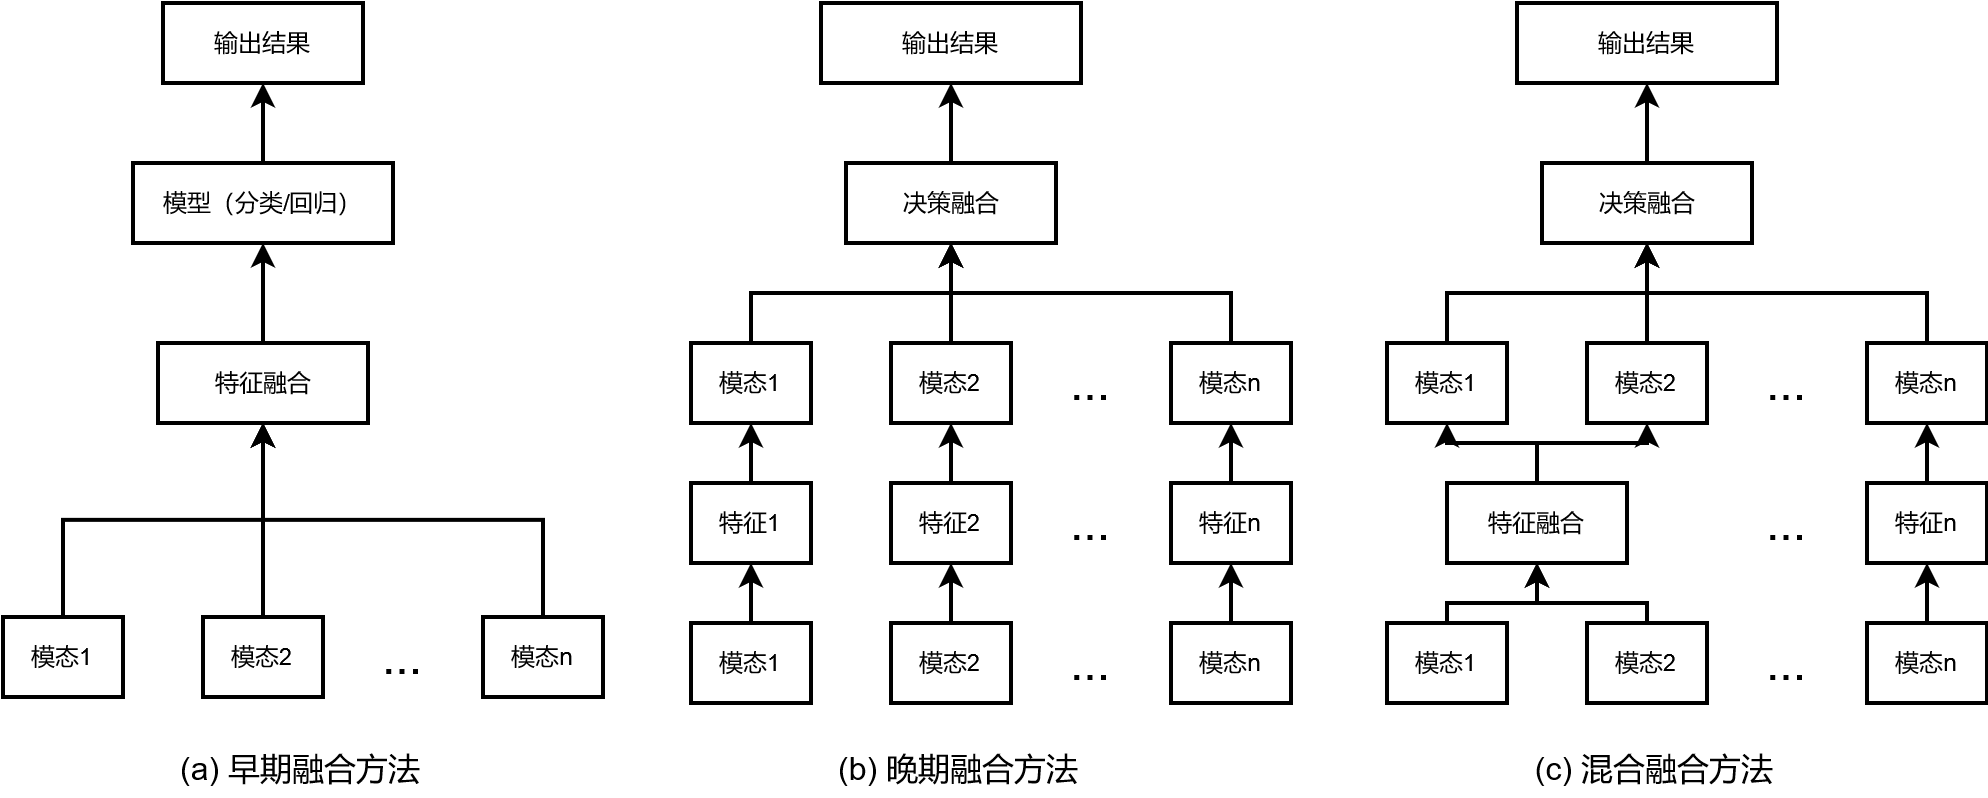
\includegraphics[width = \textwidth]{MultimodalFusion.drawio.png}
  \caption{3种多模态特征融合方法\cite{hejunandzhangcaiqing}}
  \label{fig:MultimodalFusio}
\end{figure}

早期融合的效果很大程度上依赖于对模态特性的理解和模型结构的设计,可能不适用于所有类型的多模态数据。
由于每个模态独立处理,晚期融合可能无法捕获模态之间的深层次相互作用。
而且晚期融合通常在决策层面进行,限制了对不同模态特征之间更细粒度关系的探索。
而混合融合能够通过结合早期、晚期和中间融合的优点,提供了更大的灵活性来设计模型。
这使得混合融合能够更好地适应不同模态之间的复杂关系和动态变化。
通过在不同的层级和阶段整合信息,混合融合能够最大化地利用不同模态之间的信息,包括直接的特征信息和深层次的相互作用信息。\par

\begin{figure}[htbp]
  \centering
  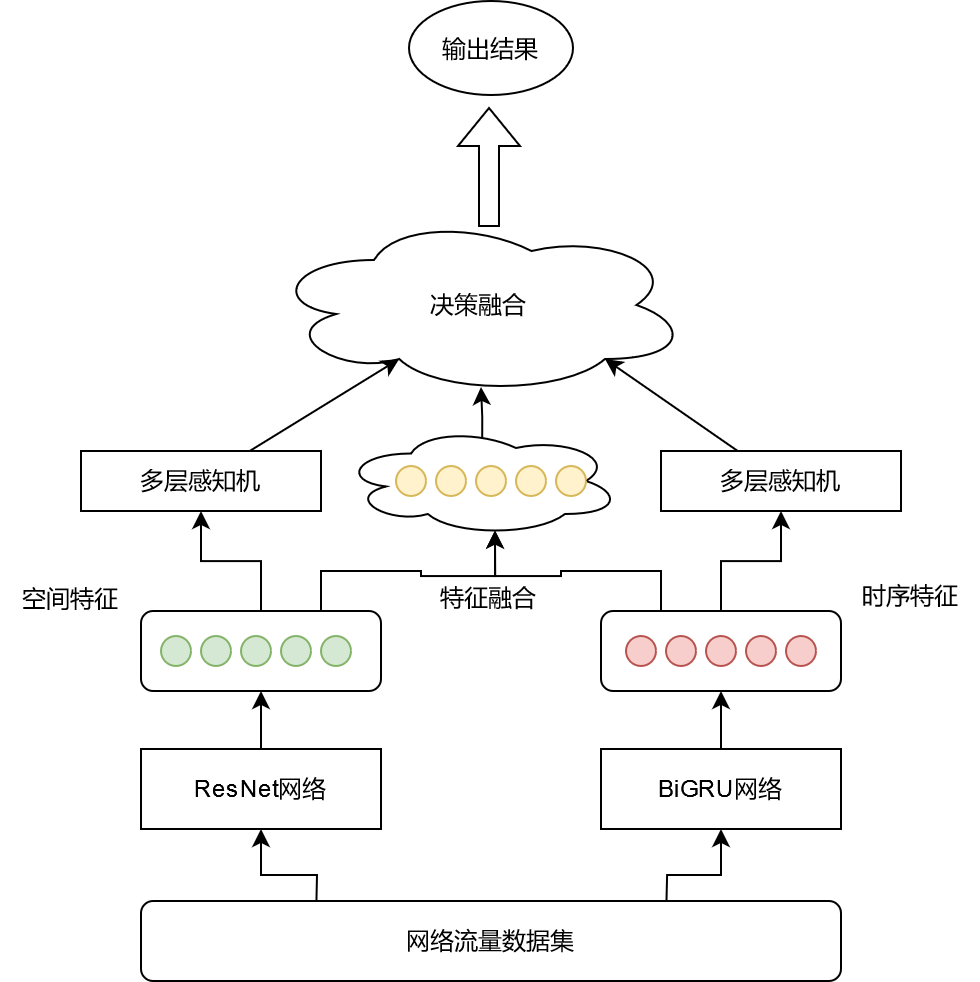
\includegraphics[width = 0.8\textwidth]{ResNet-BiGRU-Fusion.drawio.png}
  \caption{ResNet-BiGRU特征融合设计}
  \label{fig:ResNet-BiGRU-Fusion}
\end{figure}

本文将利用混合融合的方法来融合ResNet-BiGRU模型。
首先本文分别利用ResNet从网络流量数据集中提取的空间特征以及BiGRU提取时序特征,再将两个特征融合。为了简化计算量,我们使用联合架构进行融合。
联合架构有两种方法,一种是"加"联合方法。一种是"乘"联合方法。
"加"联合方法,或简称加法融合,通常指的是将不同模态的特征向量进行加权和或简单的相加操作。
这种方法假设不同模态的特征贡献可以直接相加,以形成一个综合的特征表示。
加法融合可以表示为:
\begin{equation}
  z = f(w_1^Tv_1 + w_2^Tv_2+ \dots + w_n^Tv_n)
\end{equation}
\begin{flushleft}
  \renewcommand\arraystretch{1.25}
  \begin{tabularx}{\textwidth}{@{}>{\normalsize\rm}l@{\quad}>{\normalsize\rm}l@{——}>{\normalsize\rm}X@{}}
  式中& $\symbf{z}$ &共享语义子空间的输出结果;\\
  &  $\symbf{N}$&类别总数;\\
  &  $\symbf{v}$ &各模态的输入;\\
  &  $\symbf{w}$ & 权重,下标表示不同的模态,通过映射$f$将所有子模态语义转换到共享子空间。\\
  \end{tabularx}\vspace{.5ex}%TODO : 注释内容自动转页接排
  \end{flushleft}


  "乘"联合方法,或乘法融合,涉及到对不同模态的特征进行乘积操作。
  这种方法基于这样的假设:一个模态的特征可以通过与另一模态的特征进行乘积来增强或抑制重要的信号。
  乘法联合可以用以下公式表示:
\begin{equation}
  z = \begin{bmatrix}v^1 \\1\\\end{bmatrix} \otimes \begin{bmatrix}v^2 \\1\\\end{bmatrix} \otimes \dots \otimes \begin{bmatrix}v^n \\1\\\end{bmatrix}
\end{equation}  
\begin{flushleft}
  \renewcommand\arraystretch{1.25}
  \begin{tabularx}{\textwidth}{@{}>{\normalsize\rm}l@{\quad}>{\normalsize\rm}l@{——}>{\normalsize\rm}X@{}}
  式中& $\symbf{z}$ &融合张量后的结果输出;\\
  &  $\symbf{v}$&不同的模态;\\
  &  $\symbf{\otimes}$ &外积算子。\\
   \end{tabularx}\vspace{.5ex}%TODO : 注释内容自动转页接排
\end{flushleft}



尽管“加”联合方法简单且容易实现,但其特征向量语义组合容易造成后期语义丢失,使模型性能降低,而“乘”联合方法弥补了这一不足,通过张量计
算使特征语义得到充分融合\cite{hejunandzhangcaiqing}。因此本文会用“乘”的方式来进行融合。
最终本文所采用的融合架构如~~\ref{fig:ResNet-BiGRU-Fusion}~所示。

\subsection{模型网络结构设计}
混合模型主要由一个残差网络模型以及双向门控循环单元网络融合而成。
其中,残差模型主要包括两种类型的残差块:conv\_block(卷积残差块)和identity\_block(恒等残差块)。
这两种块的设计理念是为了解决深度网络中的梯度消失问题,从而使网络能够在增加深度的同时保持训练的有效性和稳定性。
conv\_block负责调整输入特征图的维度,以匹配块输出时的维度变化。
它通过在残差路径中引入具有步长的卷积操作来实现降维,并通过额外的卷积层来调整通道数,从而使得主路径上的特征图尺寸与残差路径上的输出能够相匹配。
这种设计使得网络能够在增加深度的同时,适应更高层的特征表示。
identity\_block则在不需要改变输入特征图维度时使用,主要用于网络的深层部分,用以加深网络深度提高模型的性能。\par

残差模型以15x15\footnote{经过特征编码阶段后,数据的维度变为了(214,1),为了能够进行2D卷积操作,本文将数据的形状调整为(15,15,1),并进行了零填充。}的二维输入数据开始,紧接着是一个初始卷积层,该层使用64个3x3大小的滤波器,并应用’same’填充,以保持输出特征图的尺寸。
此外,这一层使用L2正则化以防止过拟合,并通过批归一化(BatchNormalization)和ReLU激活函数对特征进行标准化和非线性化处理。

接下来,模型通过两个阶段的残差块处理特征:

\begin{itemize}
  \item 第一阶段包括一个卷积残差块(conv\_block),用于调整特征图的尺寸和深度,以及一个恒等残差块(identity\_block),以在不改变特征图维度的情况下加深模型。
  \item 第二阶段同样起始于一个卷积残差块,用于进一步特征调整,然后是两个恒等残差块,用于增强模型的特征提取能力。
\end{itemize}

每个卷积残差块中的卷积层均配备L2正则化,并且所有残差块后都紧随批归一化和ReLU激活。
此设计旨在通过残差连接促进更深层网络的有效训练,避免梯度消失或爆炸问题。
在经过残差块系列处理后,模型使用平均池化层(AveragePooling2D)来减小特征图的尺寸,随后是一个Dropout层,以0.5的比率随机断开输入单元,减少过拟合风险。
最后,模型展平处理后的特征,为后续与双向门控循环单元(BiGRU)的特征融合做准备。值得注意的是,该结构在最终未直接加入全连接层,是因为设计上考虑将残差网络的空间特征与BiGRU的时序特征进行混合融合,


\begin{table}[htbp]
  \label{tab:resnet_description}
  \caption{The architecture of our simplified ResNet model}
  \centering
  \begin{tabular}{c|c|c}
    \hline
  Layer name & Output size & ResNet-BiGRU \\
  \hline
  conv1 & $15 \times 15$ & $3\times3$, 64, stride 1 \\
  \hline
  % 使用multirow和mbox命令来确保矩阵居中
  \multirow{4}{*}{conv2\_x} & \multirow{4}{*}{\centering $8 \times 8$} &
  \multirow{4}{*}{$\left[\begin{array}{c}
      1 \times 1, 64 \\
      3 \times 3, 64 \\
      1 \times 1, 256 
  \end{array}\right] \times 2$ , stride 2} \\
  &&\\
  &&\\
  &&\\
  \hline
  \multirow{4}{*}{conv3\_x} & \multirow{4}{*}{\centering $8 \times 8$} &
  \multirow{4}{*}{$\left[\begin{array}{c}
    1 \times 1, 64 \\
    3 \times 3, 64 \\
    1 \times 1, 256 
  \end{array}\right] \times 2$, stride 1} \\
  &&\\
  &&\\
  &&\\
  \hline
  avg\_pool & $1 \times 1$ & AvgPool $2 \times 2$ \\
  \hline
  flatten &1,1264&  \\
  \hline
  dropout & & Dropout(0.5) \\
  \hline
  \end{tabular}
\end{table}


对于BiGRU模型,模型的第一层拥有64个单元并保留序列中每个时间步的输出。
紧接着是一个10\%的dropout层,用于减少过拟合通过随机丢弃一部分的特征连接。
之后,数据流经第二个BiGRU层,这次是32个单元,不过这一层不保留序列中每个时间步的输出,只输出最后的结果。
随后是另一个10\%的dropout层。
值得注意的是,为了将BiGRU层的特征输出与ResNet模型的特征进行合并,在这个结构中也同样并没有加入全连接层(Dense layer)作为输出。\par


最后,从ResNet模型以及BiGRU模型中分别提取决策输出,并通过Dense层进行处理,使得每个模型的输出都通过一个softmax激活函数转换成类别决策。
此外,代码中引入了一个特殊的特征处理步骤,将ResNet模型的输出从11264维映射到64维,以便与BiGRU模型的输出进行元素乘法操作,合并来自两种不同模型的信息。
随后,将ResNet和BiGRU的决策输出与经过特征乘操作的结果合并成一个统一的张量,再通过一个额外的Dense层,这一层输出最终的分类决策。

图~\ref{fig:hyber_model_struct}~是这个混合模型的整体架构,表~\ref{tab:model_params}~是混合模型的参数数量,以便于理解本文模型的架构。
\begin{figure}[htbp]
  \centering
  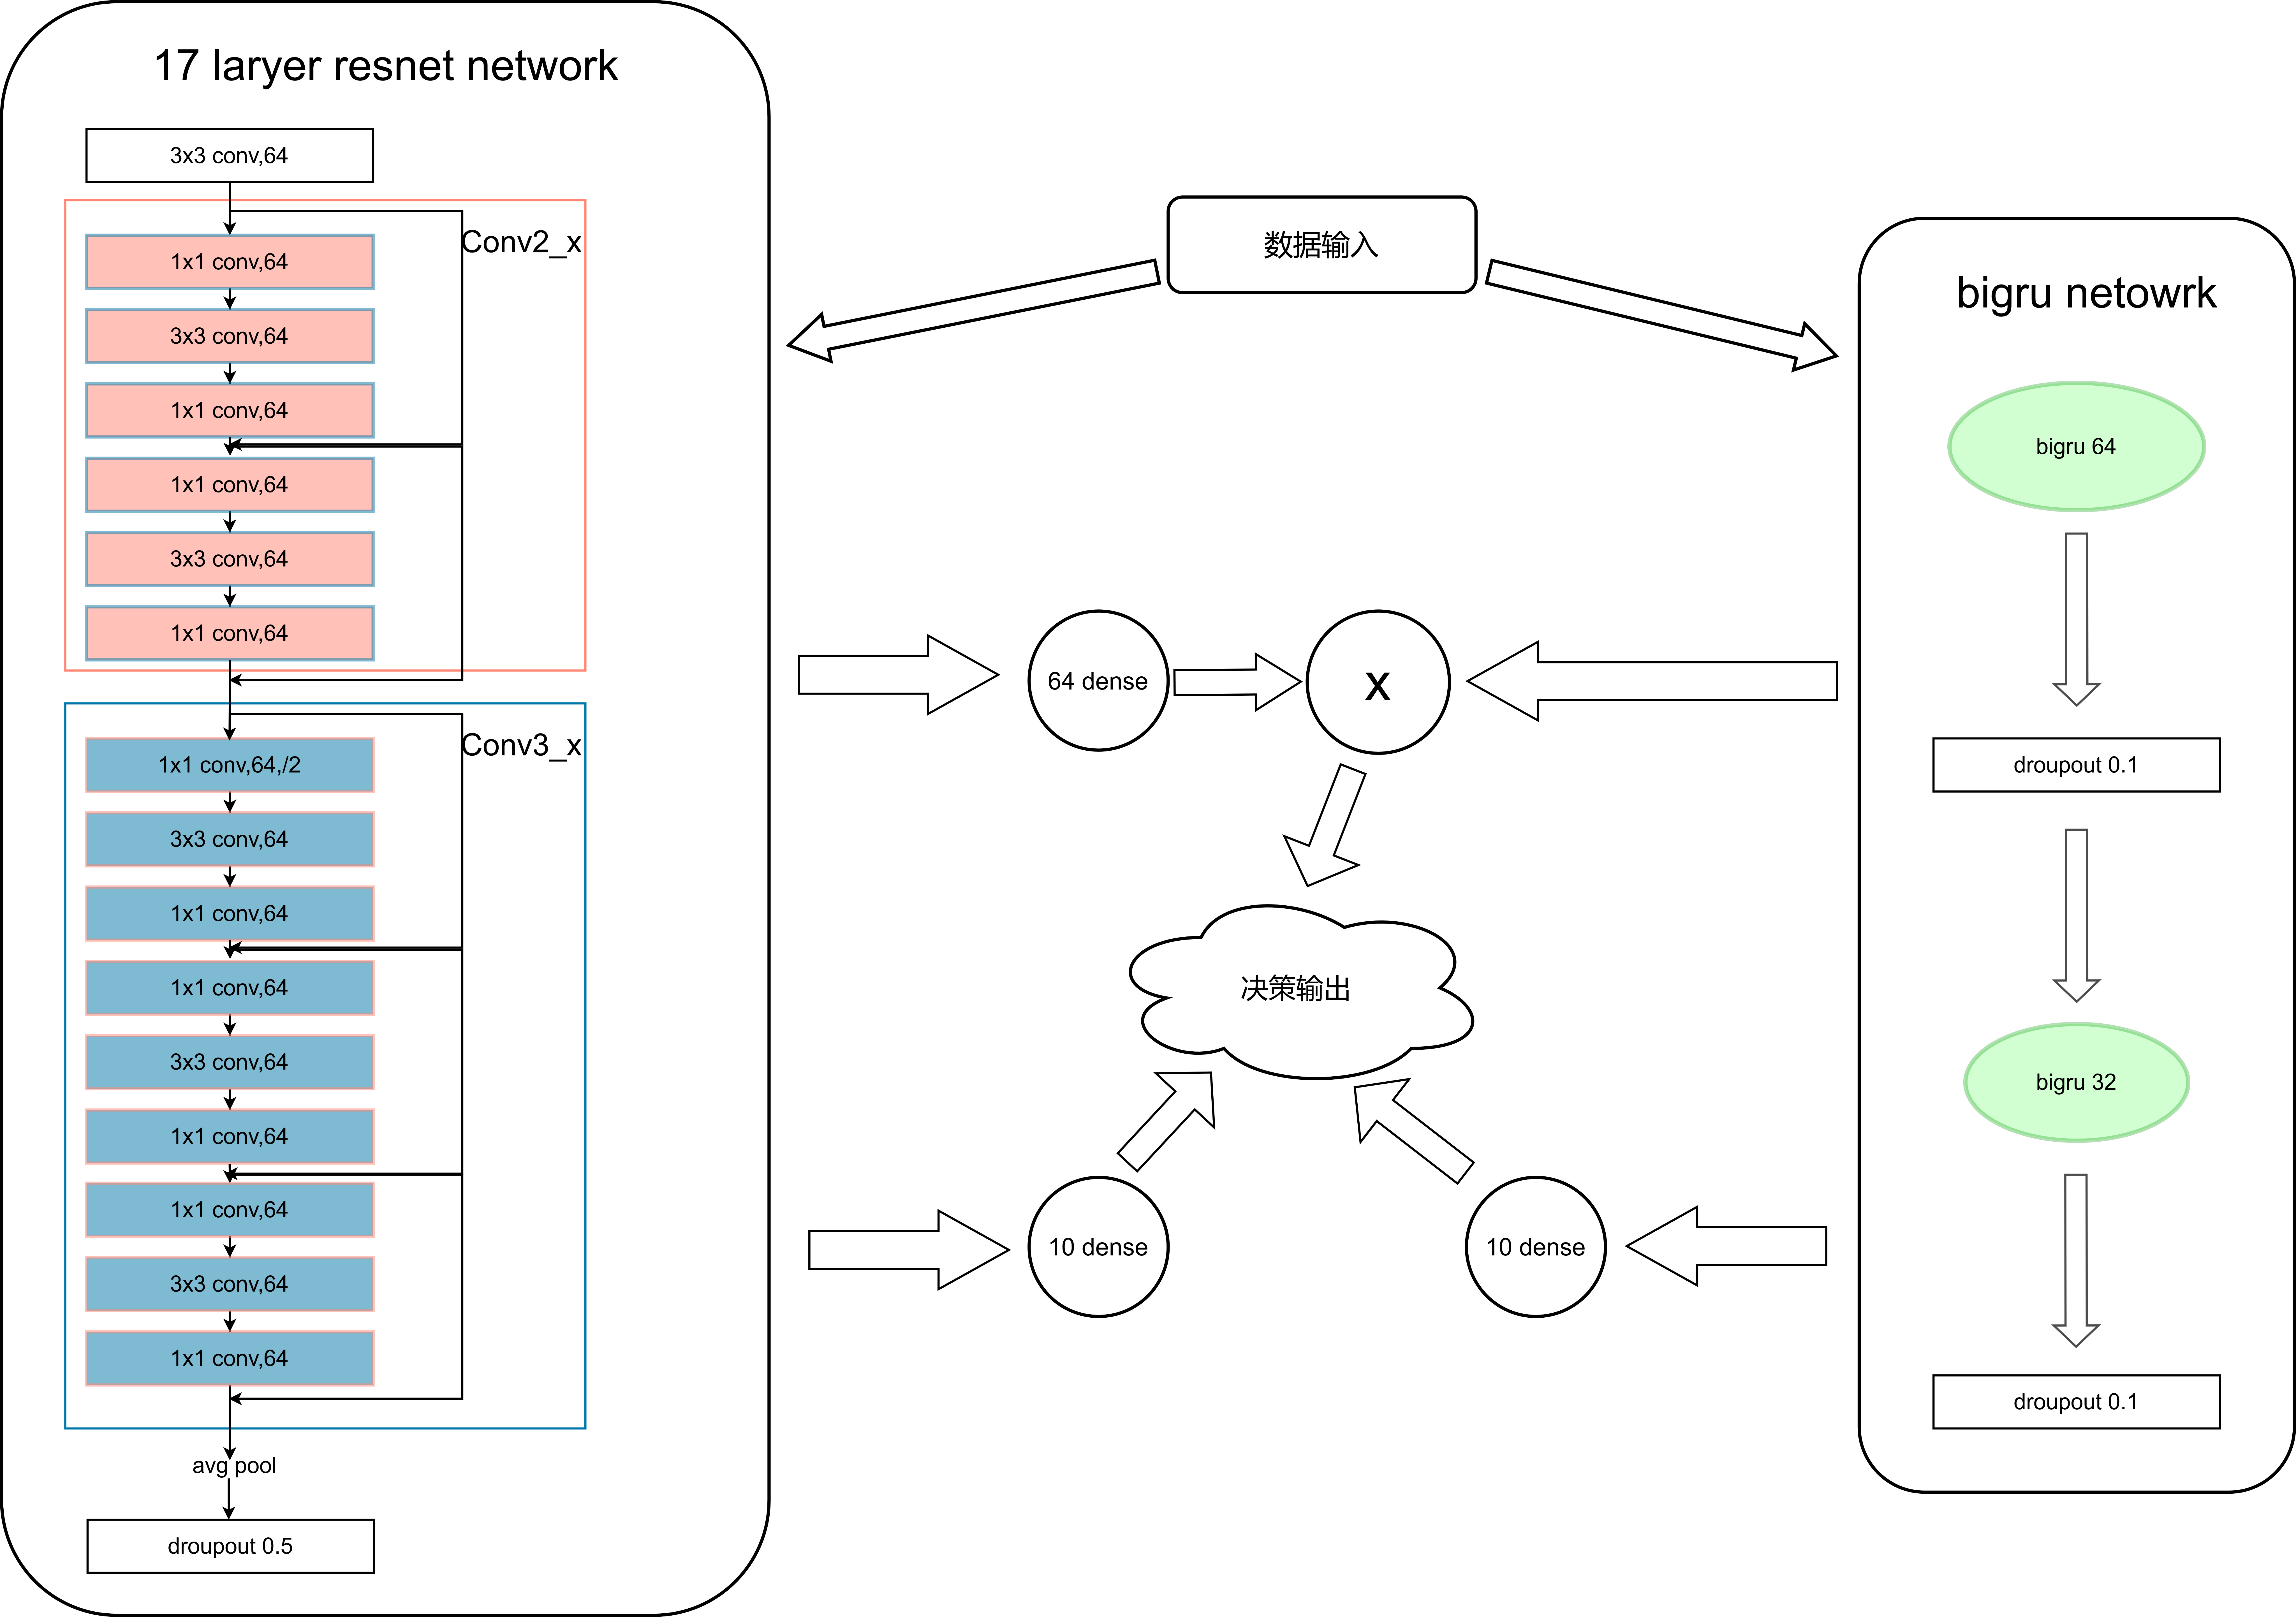
\includegraphics[width = \textwidth]{hyber_model_struction.drawio.png}
  \caption{混合模型整体结构}
  \label{fig:hyber_model_struct}
\end{figure}



\begin{table}[htbp]
  \caption{混合模型参数数量}
  \label{tab:model_params}
  \centering
  \begin{tabular}{ccc}
    \toprule
    \textbf{总参数} & \textbf{可训练参数数量} & \textbf{非可训练参数数量}\\
    \midrule
    1,417,510 & 1,412,518 & 4,992\\
    \bottomrule
  \end{tabular}
\end{table}

\section{数据预处理}
数据预处理是深度学习或机器学习一个至关重要的步骤,
进行数据预处理的目的是制作出一个干净、标准化、均衡的数据集,为特征学习和后续的模型训练打下坚实的基础。
正确的数据预处理策略可以显著提高模型的性能,加快训练速度,并提高模型在未见数据上的泛化能力。
本文在数据预处理阶段采取了综合性的方法论,旨在优化模型的学习效率和性能。\par

首先,对训练集和测试集执行特征编码,以便将分类数据转换为模型可处理的格式。
随后,本文针对原始数据集及特征编码过程中可能产生的缺失值进行了细致的处理,确保数据的完整性。
在完成上述步骤后,进一步通过特征选择技术降低数据维度,这一步骤旨在剔除冗余或不相关的特征,从而提高模型训练的效率并可能提升模型的泛化能力。
此外,对特征选择后的数据进行标准化处理,确保所有特征都在相同的尺度上,进一步促进模型学习。
鉴于本章所选用的数据集呈现显著的不平衡性,本文将会对数据集中的少数类样本进行过采样处理,以期在训练过程中实现更为均衡的类别表示和提升模型对少数类的识别能力。\par

图~\ref{fig:dataprocess}~概括性地展示了整个数据预处理和模型训练的流程。
本节接下来的部分将对这一流程中的关键步骤进行详细阐述,以便于读者深入理解本文采取的方法论及其背后的逻辑。
\begin{figure}[htbp]
  \centering
  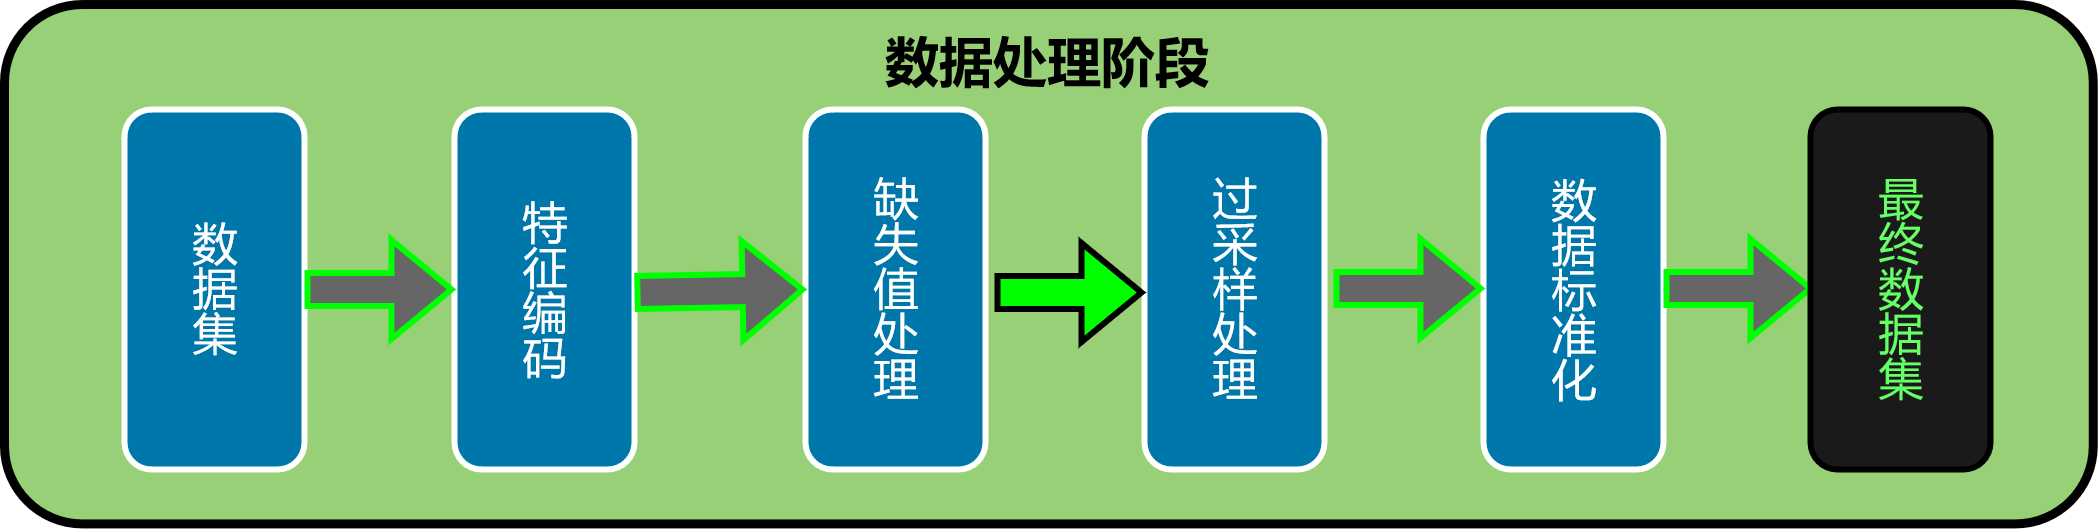
\includegraphics[width = 0.8\textwidth]{dataprocess.drawio.png}
  \caption{数据集预处理流程图}
  \label{fig:dataprocess}
\end{figure}

\subsection{特征编码}
\begin{table}[htbp]
  \caption{One-hot编码算法实现}
  \label{tab:onehot}
  \centering
  \begin{tabularx}{1.0\textwidth}{cl}
  \toprule
  \multicolumn{2}{l}{\textbf{one-hot编码算法}}\\
  \midrule
  \multicolumn{2}{l}{\textbf{输入}: 数据集 $D$,其中包含数值型和分类型列} \\ 
  \multicolumn{2}{l}{\textbf{输出}: 经过One-hot编码的数据集 $D'$} \\
  1& 初始化一个空的数据集 $D'$ \\
  2& \textbf{for} 每一列 $col$ \textbf{in} $D$: \\
  3&\quad \textbf{if} $col$ 是分类型: \\
  4&\quad\quad $unique\_values$ = 获取 $col$ 的所有唯一值 \\
  5&\quad\quad \textbf{for} 每一个值 $val$ \textbf{in} $unique\_values$: \\
  6&\quad\quad\quad 创建一个新列 $new\_col$,名称为 ``$col\_val$''\\
  7&\quad\quad\quad \textbf{for} 每一行 $row$ \textbf{in} $D$: \\
  8&\quad\quad\quad\quad \textbf{if} $row[col] == val$: \\
  9&\quad\quad\quad\quad\quad 在 $D'[new\_col]$ 中填充 1 \\
  10&\quad\quad\quad\quad \textbf{else}: \\
  11&\quad\quad\quad\quad\quad 在 $D'[new\_col]$ 中填充 0 \\
  12&\quad \textbf{else}: \\
  13&\quad\quad 将 $col$ 直接复制到 $D'$ 中 \\
  14&\textbf{return} $D'$ \\ 
  \bottomrule
  \end{tabularx}
  \end{table}
特征编码是一种数据预处理方法,用于将原始数据转换为机器学习算法能够理解和处理的格式。
这个过程对于提高模型的性能和准确性至关重要,因为大多数机器学习算法预期输入数据为数值型,而原始数据往往包括各种类型,如文本、日期或分类数据。
特征编码操作的目的便是将非数值特征转换为数值形式,使算法能够对这些数据进行计算。
因为我们的流量数据集中也存在着许多非数值类型的特征(例如:IP地址、协议类型等),所以我们这里也需要对数据集进行特征编码,将非数值类型转为数值类型。\par


One-Hot 编码是一种特殊且广泛使用的特征编码方法,它易于理解和实现,非常适用于处理具有有限类别的分类数据。
因此本文将选用one-hot编码方法对数据集中的非数值类型进行特征编码。
这种编码方法通过为每个类别创建一个新的二进制列来工作。
对于每个数据点,它所属的类别的列被标记为1,而所有其他列被标记为0。
表~\ref{tab:onehot}~是本文采用one-hot编码对数据集进行特征编码的具体算法。\par


在处理IP地址时,直接进行One-Hot编码会破坏其内在特征并导致维度爆炸,影响模型性能。
常见的处理方法包括字段分割、整数转换、地理定位和嵌入法。字段分割法将IPv4地址拆分为四个数值特征,保留模式识别能力。
整数转换法将IP转为32位整数(IPv6为更大整数),保持层次结构,适合数值特征处理。
地理定位将IP映射到地理特征,如国家、城市,利用外部服务获取,适用于地域分析。
嵌入法通过深度学习将IP转换为向量,捕获地址间相似性,但计算成本高。
考虑到整数法可能引起特征不平衡,地理定位操作复杂,嵌入法计算代价大,本文采用字段分割法简化处理流程。

\subsection{数据集平衡处理}
在大规模数据集预处理中,解决数据不平衡问题是提高模型性能和泛化能力的关键步骤。
通过图~\ref{fig:kddtraindistribution}、\ref{fig:kddtestdistribution}和\ref{fig:UNSW-NB15barchart}~明显可以看出,本文采用的数据集是非常不均衡的,因此本文将会对数据集进行平衡处理。
数据不平衡通常通过欠采样和过采样两种重采样策略来处理。
欠采样通过减少多数类样本来达到平衡,尽管可能丢失一些信息,但有助于增强模型对少数类的关注。
相反,过采样则通过增加少数类样本数量来平衡数据,例如可以采用复制样本或利用SMOTE等高级技术生成新样本,提高少数类的代表性。
在样本量不足时,过采样尤为适用,鉴于此,本文将会利用SMOTE算法对数据集进行平衡处理。\par


SMOTE(Synthetic Minority Over-sampling Technique,合成少数类过采样技术)是一种被广泛采用的过采样策略,旨在通过合成新的少数类样本而非简单重复现有样本来增强数据集的类别平衡。
此技术显著提升了分类器对少数类的识别能力,进而改善了模型的整体性能及其泛化能力。
SMOTE算法的核心优势在于其能够通过引入合成样本增加数据集的多样性,促进模型学习更复杂的决策边界\cite{chawla2002smote}\cite{fernandez2018smote}。
表~\ref{tab:smote}~是该技术的算法实现。
\begin{table}[htbp]
  \caption{SMOTE算法实现}
  \label{tab:smote}
  \centering
  \begin{tabularx}{1.0\textwidth}{cl}
  \toprule
  \multicolumn{2}{l}{\textbf{SMOTE算法}}\\
  \midrule
  \multicolumn{2}{l}{\textbf{输入}: 少数类样本集 $S$,采样倍率 $N$,最近邻数 $k$} \\ 
  \multicolumn{2}{l}{\textbf{输出}: 合成样本集 $S'$} \\
  1& 如果 $N$ 不是整数,则将 $N$ 向下取整,同时调整最终的样本数量 \\
  2& 初始化空的合成样本集 $S'$ \\
  3& \textbf{for} 每一个样本 $s$ \textbf{in} $S$: \\
  4&\quad 找到 $s$ 的 $k$ 个最近邻 \\
  5&\quad \textbf{for} $i$ \textbf{from} 1 \textbf{to} $N$: \\
  6&\quad\quad 随机选择一个最近邻 $nn$ \\
  7&\quad\quad \textbf{for} 每个特征 $f$: \\
  8&\quad\quad\quad 计算 $s$ 和 $nn$ 在特征 $f$ 上的差值 $\Delta f$ \\
  9&\quad\quad\quad 生成新值 $new\_f = s[f] + \Delta f \times \text{随机数}(0, 1)$ \\
  10&\quad\quad 创建新样本 $new\_s$,其特征值为所有生成的 $new\_f$ \\
  11&\quad\quad 将 $new\_s$ 添加到合成样本集 $S'$ \\
  12&\textbf{return} $S'$ \\ 
  \bottomrule
  \end{tabularx}
\end{table}

% 对于表~\ref{tab:smote}~中算法的最佳采样倍率,通常不能直观的获取到。
% 为了取得最优的抽样比率,本文将会利用遗传算法对采样倍率进行优化。
% 为了进一步提升模型在处理类别不平衡数据集时的性能,本文引入了一种基于遗传算法的SMOTE优化技术。
% 该技术旨在调整采样比率,以寻找合成样本中类别占比的一个理想平衡点,这个平衡点能够在增强模型对少数类识别能力的同时,避免过拟合和信息冗余的问题。
% 以下是该方法的详细介绍。\par




\section{实验评估与分析}
\subsection{实验数据集介绍}
UNSW-NB15数据集\cite{moustafa2015comprehensive}由澳大利亚新南威尔士大学的网络安全实验室开发,旨在克服以往数据集的不足并提供更实际的测试环境。
与早期的KDD Cup 99和NSL-KDD数据集相比,UNSW-NB15引入了一系列的改进和特色,以适应网络威胁检测的新要求。
这些改进体现在数据集的构成、攻击类型的多样性以及数据的实用性和代表性上。

\begin{table}[htbp]
  \caption{UNSW-NB15流量分布及其描述}
  \label{tab:UNSW-NB15_distribution}
  \begin{tabularx}{\textwidth}{@{}cccX@{}}
    \toprule
      \multicolumn{1}{c}{\textbf{种类}} & \multicolumn{1}{c}{\textbf{数量}} & \multicolumn{1}{c}{\textbf{占比(\%)}} & \multicolumn{1}{c}{\textbf{描述}}\\
    \midrule
  Normal & 2218761 & 87.35\% & 正常数据 \\

  Fuzzers & 24246 & 0.95\% & 通过向程序或网络输入随机数据尝试使其悬挂或暂停的攻击 \\

  Analysis & 2677 & 0.11\% & 包含不同的端口扫描、垃圾邮件和html文件渗透攻击 \\

  Backdoors & 2329 & 0.09\% & 一种秘密绕过系统安全机制以访问计算机或其数据的技术 \\

  DoS & 16353 & 0.64\% & 恶意尝试使服务器或网络资源对用户不可用,通常通过暂时中断或悬挂连接到互联网的主机的服务来实现 \\

  Exploits & 44525 & 1.75\% & 攻击者了解操作系统或软件内的安全问题,并利用这一点通过利用漏洞进行攻击 \\

  Generic & 215481 & 8.48\% & 一种针对所有给定块大小和密钥大小的分组密码的技术,不考虑分组密码的结构 \\

  Reconnaissance & 13987 & 0.55\% & 包含所有可以模拟收集信息攻击的攻击 \\

  Shellcode & 1511 & 0.06\% & 利用软件漏洞进行攻击的载荷中的一小段代码 \\

  Worms & 174 & 0.01\% & 攻击者复制自身以便传播到其他计算机,通常使用计算机网络传播,依赖于目标计算机上的安全漏洞进行传播 \\
  \bottomrule
  \end{tabularx}
  \end{table}

首先,UNSW-NB15数据集通过包含更现代的攻击类型,如DoS、蠕虫、后门攻击和Fuzzers等(关于具体的攻击种类详见表~\ref{tab:UNSW-NB15_class}~,数据集类别占比详见表~\ref{tab:UNSW-NB15_distribution}~和图~\ref{fig:UNSW-NB15barchart}~)。
这种多样化的攻击样本集合使得数据集不仅能够用于传统的入侵检测研究,也适用于评估面对新型攻击行为的检测系统的效果。

  
  \begin{figure}[htbp]
    \centering
    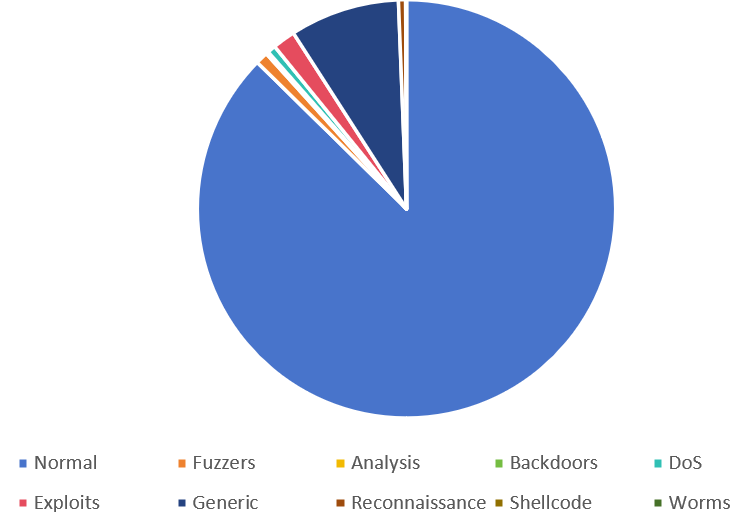
\includegraphics[width = 0.8\textwidth]{UNSW-NB15barchart.png}
    \caption{UNSW-NB15数据集分布占比饼状图}
    \label{fig:UNSW-NB15barchart}
    \end{figure}


其次,UNSW-NB15提供了四个CSV格式的数据记录文件,每个文件中都包含了攻击记录和正常记录。这些CSV文件分别命名为UNSWNB15\_1.csv、UNSW-NB15\_2.csv、UNSW NB15\_3.csv和UNSW-NB15\_4.csv。
在每个CSV文件中,所有记录都根据最后一个时间属性进行了排序。前三个CSV文件中,每个文件包含700,000条记录;第四个文件包含440,044条记录,共2,540,044条记录。


海量的数据集不仅有助于模型的训练和验证,也提高了入侵检测模型在实际环境中应用的可信度和有效性。
此外,UNSW-NB15数据集在设计时注重了实用性和代表性,通过模拟现实世界的网络环境和流量模式,确保了数据集的广泛适用性和长期价值。
这使得该数据集成为评估和比较不同入侵检测技术性能的理想选择。
\begin{table}[htbp]
  \caption{UNSW-NB15数据集中每种攻击的不同子类的细分}
  \label{tab:UNSW-NB15_class}
  \begin{tabularx}{\textwidth}{@{}ccX@{}}
  \toprule
    \multicolumn{1}{c}{\textbf{种类}} & \multicolumn{1}{c}{\textbf{数量}} & \multicolumn{1}{c}{\textbf{子类}}\\
  \midrule
    Fuzzers & 10 & FTP, HTTP, RIP, SMB, Syslog, PPTP, TFTP, DCERPC, OSPF, BGP\\
    Probe & 13 & Telnet, SNMP, SunRPC Portmapper (TCP) UDP Service, SunRPC Portmapper (TCP) TCP Service, SunRPC Portmapper (UDP) UDP Service, NetBIOS, DNS, HTTP,
    SunRPC Portmapper (UDP), ICMP, SCTP, MSSQL, SMTP\\
    Shellcode & 15 & FreeBSD, HP-UX, NetBSD, AIX, SCO Unix, Linux, Decoders, IRIX, OpenBSD, Mac OS X, BSD, Windows, BSDi, Multiple OS, Solaris\\
    Analysis & 3 & HTML, Port Scanner, Spam\\
    Backdoors & 1 & Backdoors\\
    DoS & 36 & Ethernet, SunRPC, LDAP, Browser, DCERPC, Telnet, NetBIOS/SMB, DNS, TCP, Common Unix Print System (CUPS), Miscellaneous, ISAKMP, Hypervisor, 
    Cisco Skinny, IIS Web Server, IGMP, ICMP, XINETD, SIP, RTSP, Windows Explorer, IRC, NTP, CUPS, Asterisk, HTTP, Microsoft Office, SSL, IMAP, SMTP, Oracle, RDP, VNC, FTP, TFTP, SNMP\\
    Exploits & 54 &Clientside Microsoft Paint, Dameware, Clientside Microsoft Media Player, SSH, SCCP, Unix r Service, SunRPC, LDAP, Web Application, Browser, DCERPC, Interbase, Telnet, DNS, TCP, Webserver, SCADA, SMB, Miscellaneous, Cisco IOS, All, LPD, RADIUS, RDesktop, Unix 'r' Service, IGMP, POP3, ICMP, Clientside Microsoft, Microsoft IIS, Backup Appliance, IDS, Apache, NNTP, RTSP, Evasions, SIP, WINS, Office Document, PHP, Clientside Microsoft Office, Miscellaneous Batch, Browser FTP, MSSQL, SOCKS, PPTP, Clientside, SSL, IMAP, SMTP, Oracle, VNC, FTP, TFTP\\
    Generic& 7 &All,SIP,HTTP,SMTP,IXIA,TFTP,Superflow\\
    Reconnaissance& 14 &DNS, HTTP, ICMP, MSSQL, NetBIOS, SCTP, SMTP, SNMP, SunRPC, SunRPC Portmapper (TCP) TCP Service, SunRPC Portmapper (TCP) UDP Service, SunRPC Portmapper (UDP) TCP Service, SunRPC Portmapper (UDP) UDP Service, Telnet\\
    Worms&1&Worms\\
    \bottomrule
  \end{tabularx}
\end{table}
\subsection{实验环境}
为了评估本文所提方案的有效性,本文将利用python语言来实现以上流程,并选用表~\ref{tab:env_setting}~中的配置来进行实验。

\begin{table}[htbp]
  \caption{实验设备配置}
  \label{tab:env_setting}
  \centering
  \begin{tabular}{ccc}
    \toprule
    \textbf{环境类别} & \textbf{设备项目} & \textbf{项目参数}\\
    \midrule
    \multirow{6}{*}{硬件环境}& CPU型号 & Intel(R) Core(TM) i7-11800H\\
                            & CPU规格 & 8核16线程@2.30GHz\\
                            & GPU型号 & NVIDIA GeForce RTX 3060 Laptop GPU\\
                            & 内存大小& 16.0 GB\\
                            & 硬盘类型& SSD\\
                            & 硬盘大小& 1TB\\
                            \hline
    \multirow{3}{*}{软件环境}&操作系统&Windows 11\\
                            &开发语言&Python 3.11.7\\
                            &编辑器 &Visual Studio Code\\                       
    \bottomrule
  \end{tabular}
\end{table}

\subsection{评估指标}
本文主要使用准确度 (Accuracy)、精确度 (Precision)、召回率 (Recall)、加权平均 F1 分数 (Macro Averaged F1 Score)、宏平均 F1 分数 (Macro Averaged F1 Score)这5个评价指标对我们的方案进行全方位的评估。
以下是这5个指标的简单介绍。\par
(1) 准确度\par
表示模型正确预测的比例,是所有正确预测的数量除以总预测数量。
\begin{equation}
  \label{eq:val_score1}
  Accuracy = \frac{Number of Correct Predictions}{Total Number of Predictions} = \frac{TP + TN}{TP + TN + FP + FN}
\end{equation}

(2) 精确度\par
简称精度,也称为查准率,是所有模型预测为正类的样本中,实际为正类的比例。
\begin{equation}
  \label{eq:val_score2}
  Precision = \frac{TP}{TP + FP}
\end{equation}

(3) 召回率\par
召回率,也称为真正率、查补率,是模型正确识别为正类的样本占所有实际正类样本的比例。
\begin{equation}
  \label{eq:val_score3} 
  Recall = \frac{TP}{TP + FN}
\end{equation}

% (4) F1 分数\par
% F1 分数是精确度和召回率的调和平均,用于衡量模型的精确度和召回率的平衡程度。
% \begin{equation}
%   \label{eq:val_score4}
%   F1 = 2 \times \frac{Precision \times Recall}{Precision + Recall} = \frac{2TP}{2TP + FP + FN}
% \end{equation}

(4)宏平均 F1 分数\par
宏平均 F1 分数是一种性能评估指标,用于衡量模型在所有类别上的平均表现。
它通过简单地计算所有类别 F1 分数的算术平均值得出,每个类别被赋予相同的权重,不论其样本量大小。

\begin{equation}
 \label{eq:val_score4}
F1_{macro} = \frac{1}{N} \sum\limits_{i=1}^{N} F1_i
\end{equation}
\begin{flushleft}
  \renewcommand\arraystretch{1.25}
  \begin{tabularx}{\textwidth}{@{}>{\normalsize\rm}l@{\quad}>{\normalsize\rm}l@{——}>{\normalsize\rm}X@{}}
  式中& $\symbf{F1_{macro}}$ &表示宏平均 F1 分数;\\
  &  $\symbf{N}$&类别总数;\\
  &  $\symbf{F1_i}$ & 表示第 $i$ 个类别的 F1 分数。\\
  \end{tabularx}\vspace{.5ex}%TODO : 注释内容自动转页接排
\end{flushleft}

宏平均 F1 分数特别适用于样本分布不均匀的数据集,因为它给每个类别分配了同等的重要性。
这样做确保了即使某些类别的样本数量很少,它们在计算平均分数时也会有相等的影响。

(5) 加权平均 F1 分数\par
加权平均F1分数是一种性能评估指标,通过根据每个类别的样本量对其F1分数进行加权平均,以反映所有类别的整体性能。
每个类别的重要性通过其在数据集中的相对比例来确定。

\begin{equation}
  \label{eq:val_score5}
  F1_{weighted} = \sum\limits_{i=1}^{N} w_i \cdot F1_i
\end{equation}
\begin{flushleft}
  \renewcommand\arraystretch{1.25}
  \begin{tabularx}{\textwidth}{@{}>{\normalsize\rm}l@{\quad}>{\normalsize\rm}l@{——}>{\normalsize\rm}X@{}}
  式中& $\symbf{F1_{weighted}}$ &加权平均F1分数;\\
  &  $\symbf{N}$&类别总数;\\
  &  $\symbf{F1_i}$ &第$i$个类别的F1分数\\
  &  $\symbf{w_i}$ & 第$i$个类别的权重,通常由该类别的样本数量占总样本数量的比例确定。\\
  \end{tabularx}\vspace{.5ex}%TODO : 注释内容自动转页接排
  \end{flushleft}

% (6) 混淆矩阵\par
% 混淆矩阵是一种特定的表格布局,用于可视化模型性能,显示实际类别与模型预测类别之间的关系。
% \begin{equation}
%   \label{eq:val_score6}
%   Confusion Matrix = \begin{bmatrix} TP & FP \\ FN & TN \end{bmatrix}
% \end{equation}

% (7) ROC-AUC 分数\par
% ROC-AUC 分数是接收者操作特征(ROC)曲线下面积的度量,用于评估分类器的预测能力。
% \begin{equation}
%   \label{eq:val_score7}
%   AUC = \int_{0}^{1} TPR(FPR) \, d(FPR)
% \end{equation}

以上五式\ref{eq:val_score1}、\ref{eq:val_score2}、\ref{eq:val_score3}、\ref{eq:val_score4}、\ref{eq:val_score5}%\ref{eq:val_score6}、\ref{eq:val_score7}%
中,
  $TP$(True Positives)表示正确地将正类预测为正类;
  $TN$(True Negatives)表示正确地将负类预测为负类;
  $FP$(False Positives)表示错误地将负类预测为正类;
  $FN$(False Negatives)表示错误地将正类预测为负类。

\subsection{特征编码效果实验评估}

  在本次实验中,我们通过比较了特征编码前后各种机器学习和深度学习模型的准确率(图~\ref{fig:comapre_accuracy_encoding}~以及表~\ref{tab:model_performance}\footnote{由于表格长度有限,朴素贝叶斯的表现我们没有放到表格中,朴素贝叶斯特征编码前后各性能指标变化:Acc 97.72\% \rightarrow 97.27\% ,f1\_mac 0.3376 \rightarrow 0.2166, f1\_wei 0.9726 \rightarrow 0.9729。}
  ~),得出了一些发现。
  \begin{figure}[htbp]
    \centering
    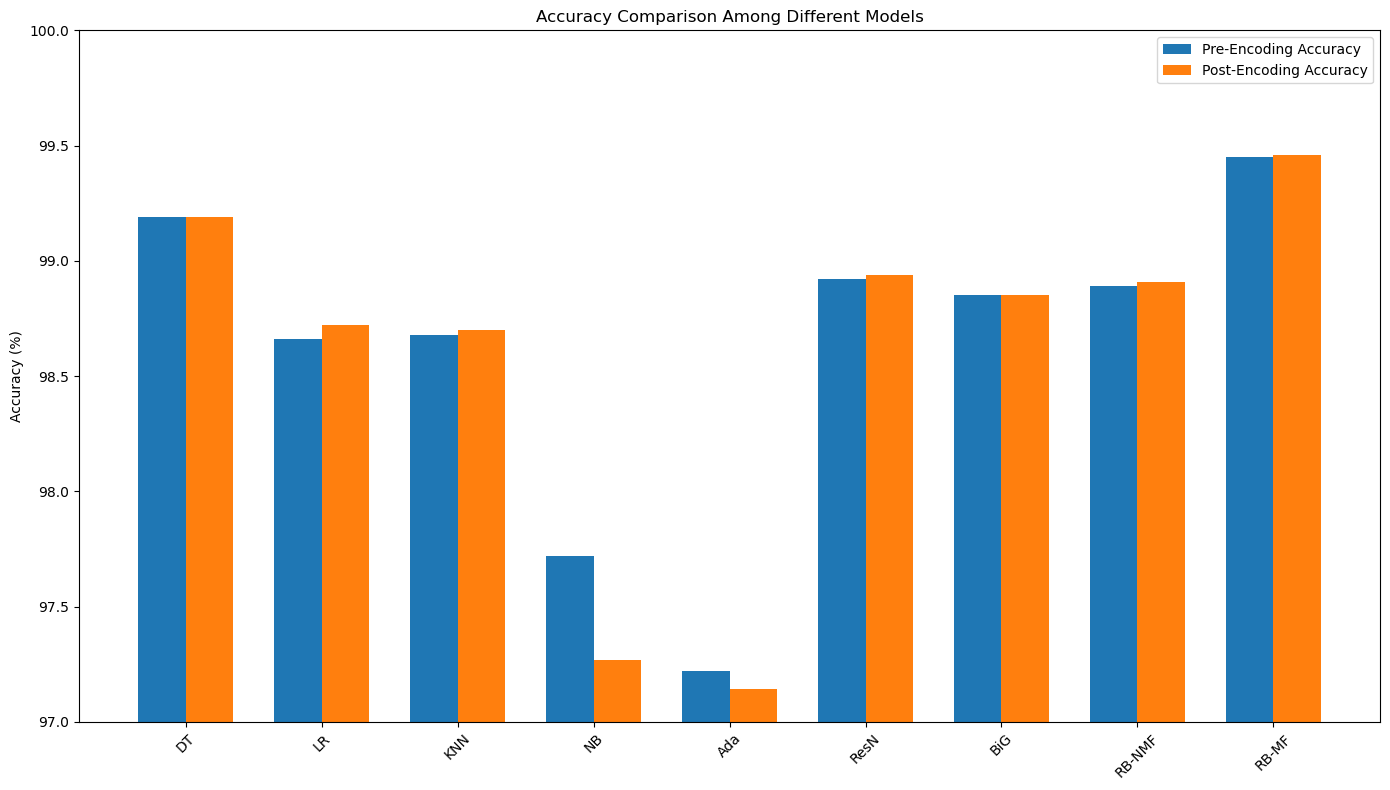
\includegraphics[width = \textwidth]{acc.png}
    \caption{特征编码前后模型预测准确率对比条状图}
    \label{fig:comapre_accuracy_encoding}
    \end{figure}
    首先,决策树模型显示出了对输入数据表示形式的鲁棒性,其准确率在特征编码前后保持不变。而逻辑回归和K近邻这样的模型则在特征编码后显示出了轻微的准确率提升,暗示了特征编码对于这类模型可能带来的轻微性能改进。
  相反,朴素贝叶斯模型在特征编码后的准确率却明显下降,可能是由于特征编码改变了数据的分布假设,从而对基于概率的模型产生了较大影响。
  深入到深度学习模型,ResNet和BiGRU在特征编码后展现出准确率的稳定提升,这可能归因于这些模型能够从编码后的特征中学习到更加复杂和深层的数据表示。
  特别值得注意的是,采用\textbf{模态特征融合策略的ResNet-BiGRU模型},在特征编码前后都表现出了所有模型中最高的准确率,尤其是在特征编码后,其准确率达到了的99.46\%,凸显了模态融合在提高模型处理能力方面的显著优势。\par
  \begin{figure}[htbp]
    \centering
    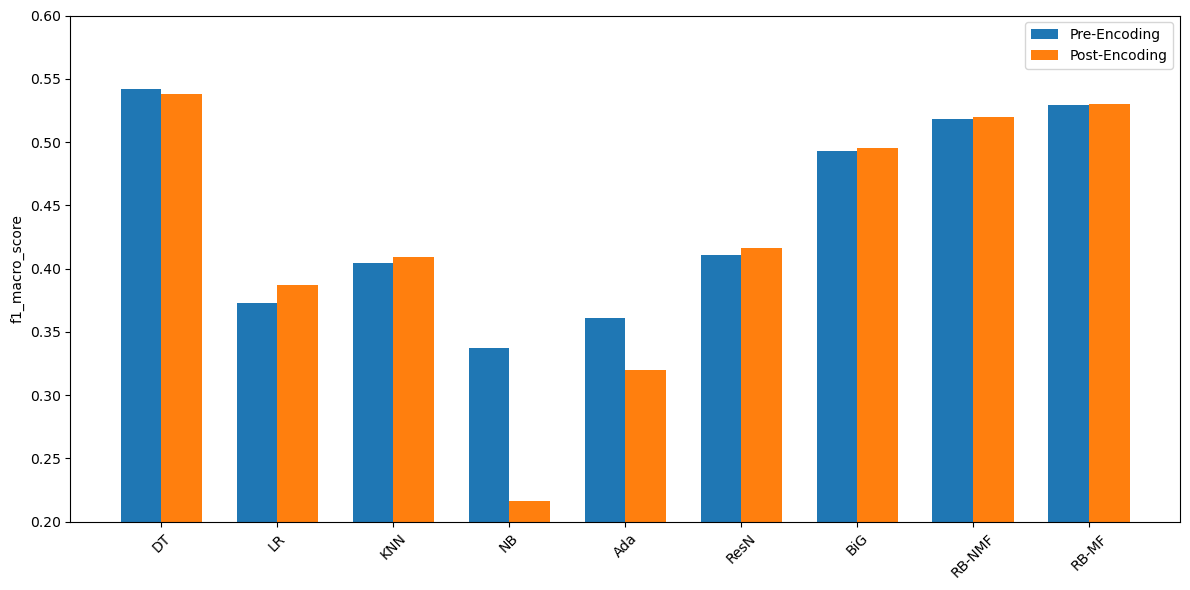
\includegraphics[width = \textwidth]{f1-mac.png}
    \caption{特征编码前后模型f1 macro score对比条状图}
    \label{fig:f1_macro_score}
    \end{figure}
  \begin{figure}[htbp]
    \centering
    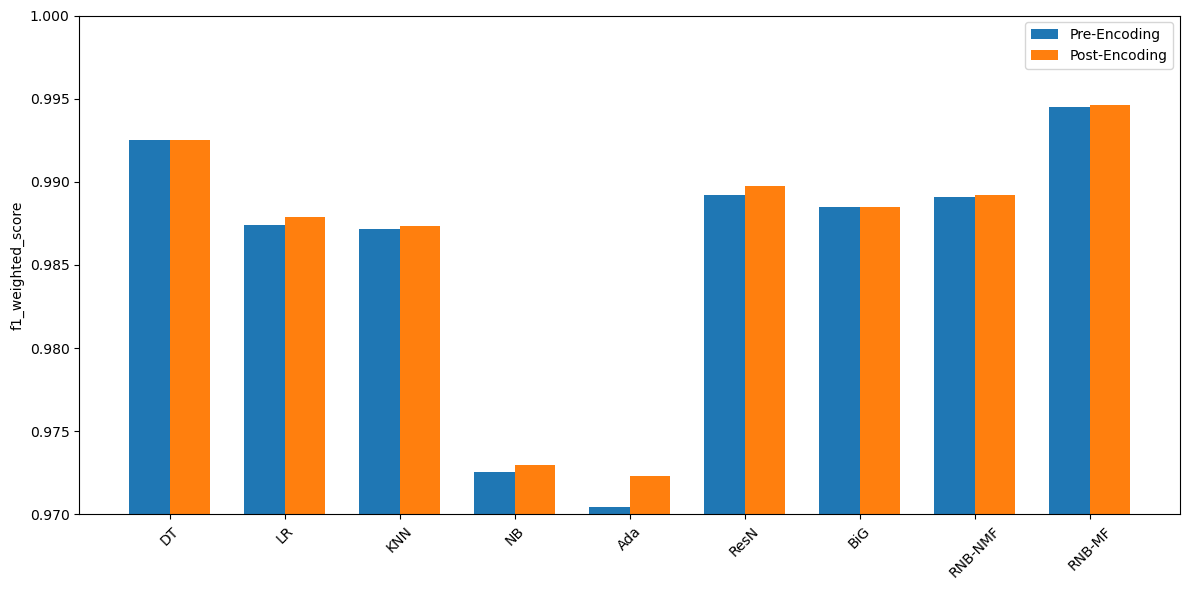
\includegraphics[width = \textwidth]{f1-wei.png}
    \caption{特征编码前后模型f1 weighted score对比条状图}
    \label{fig:f1_weighted_score}
\end{figure}

\begin{table}[htbp]
  \centering
  \caption{特征编码前后模型表现}
  \label{tab:model_performance}
  \begin{tabular}{ccccccccc}
  \toprule
  & DT & LR & KNN & Ada & ResN & BiG & RNB-NMF& RNB-MF\\
  \midrule
  \multicolumn{9}{c}{\textbf{特征编码前}}\\
  Acc & 99.19\% & 98.66\% & 98.68\%  & 97.22\% & 98.92\% & 98.85\% & 98.89\% & 99.45\% \\
  f1\_mac & 0.5422 & 0.3730 & 0.4042  & 0.3609 & 0.4110 & 0.493 & 0.518 & 0.529 \\
  f1\_wei & 0.9925 & 0.9874 & 0.9872  & 0.9704 & 0.9892 & 0.9885 & 0.9891 & 0.9945 \\
  \midrule
  \multicolumn{9}{c}{\textbf{特征编码后}}\\
  Acc & 99.19\% & 98.72\%\uparrow & 98.70\%\uparrow  & 97.14\%\downarrow & 98.94\%\uparrow & 98.85\% & 98.91\%\uparrow & 99.46\%\uparrow \\
  f1\_mac & 0.5378\downarrow & 0.3871\uparrow & 0.4090\uparrow  & 0.3197\downarrow & 0.4166\uparrow & 0.495\uparrow & 0.52\uparrow & 0.53\uparrow \\
  f1\_wei & 0.9925 & 0.9879\uparrow & 0.9873\uparrow  & 0.9723\uparrow & 0.9898\uparrow & 0.9885 & 0.9892\uparrow & 0.9946\uparrow \\
  \bottomrule
  \end{tabular}
\end{table}
整体而言,所有模型在准确率方面都表现出较高的水平,特别是在特征编码后,大多数模型的准确率略有提升,说明特征编码对模型性能有正面影响。
具体到F1分数,F1 Macro(图~\ref{fig:f1_macro_score}~)和F1 Weighted(图~\ref{fig:f1_weighted_score}~)分数在特征编码后也显示出类似的趋势。
在深度学习模型方面,ResNet和BiGRU表现出了较好的性能提升,尤其是在特征编码后,这可能归因于深度学习模型能够从编码后的特征中学习到更加复杂的表示。
同样值得注意的是,采用\textbf{模态融合策略的ResNet-BiGRU模型}在所有评价指标上都表现最优,无论是在特征编码前还是编码后。
通过观察完数据后,我们可以看到特征编码和模型选择对于提升模型性能具有重要意义。
模态特征融合技术尤其在提高复杂模型的准确率和F1分数方面显示出显著的优势,这为未来在模型设计和特征工程方面的研究提供了有价值的参考。\par

\subsection{数据集平衡处理效果实验评估}
在处理网络流量数据时,一个常见的挑战是数据的不平衡性。特别是在网络安全领域,正常流量的样本远多于异常或攻击流量的样本。
例如,本章所使用到的数据集种正常流量占总样本的87\%,这意味着即使一个模型将所有流量都预测为正常流量,其准确率也能达到87\%。
然而,这种模型对于检测异常流量来说是无效的,因为它无法识别出任何异常样本,这显然不是我们期望的结果。\par


\begin{table}
  \centering
  \caption{数据集平衡处理前后数据量变化}
  \label{tab:attack_num}
\begin{tabular}{ccc}
\toprule
\textbf{攻击类型}&\textbf{过采样前}&\textbf{过采样后}\\
\midrule
Fuzzers&3775&50844\\
Analysis&382&50844\\
Backdoors&400&50844\\
DoS&879&50844\\
Exploits&4038&50844\\
Generic&5587&50844\\
Reconnaissance&1316&50844\\
Shellcode&164&50844\\
Worms&18&50844\\
normal&508447&508447\\
  % 2 4 8 16 32 64 128
  %        104  96
  %        108  112
  %        110
  %        111
  \bottomrule
\end{tabular}
  
\end{table}
\begin{figure}[htbp]
  \centering
  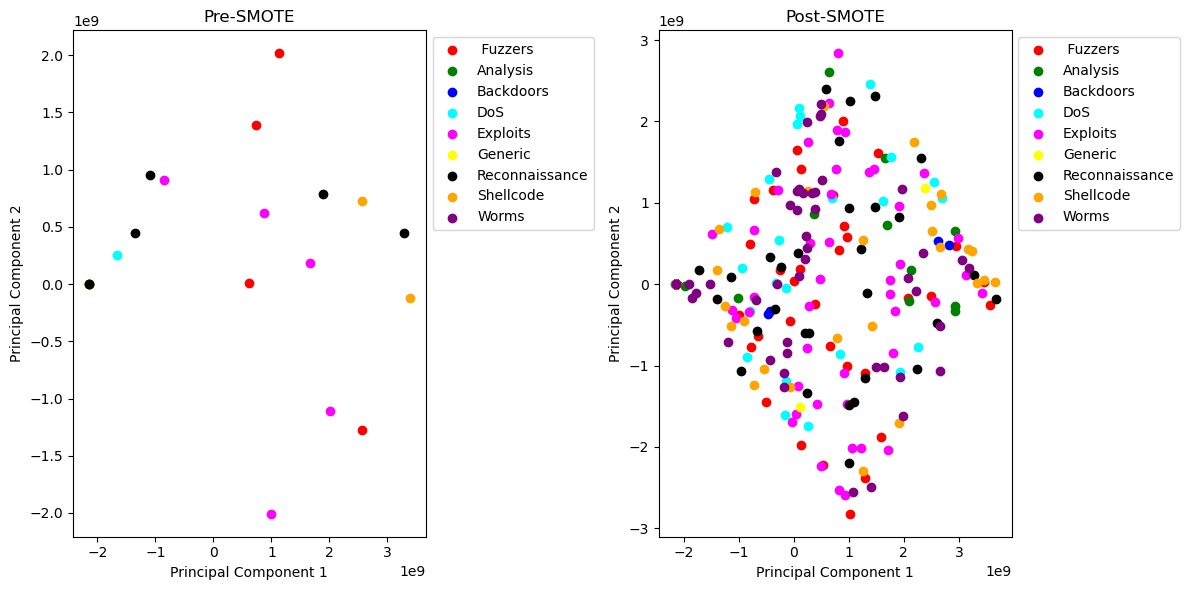
\includegraphics[width = \textwidth]{smote.png}
  \caption{SMOTE过采样前后,1000个样本中各种攻击类别的样本点变化,这里省略了normal样本点}
  \label{fig:prepostsmote}
\end{figure}

为了解决这一问题,我们采用了SMOTE算法对异常样本进行过采样。
通过这种方法,我们能够增加异常流量样本的数量,从而改善训练数据的平衡性。
过采样的结果如表~\ref{tab:attack_num}所示,从中可以看出,过采样后各类样本的数量有了明显的变化。
此外,我们使用PCA(主成分分析)方法将样本降维到2D平面上,并在图~\ref{fig:prepostsmote}中展示了过采样前后的情况。
从图中可以清晰地看到,攻击样本的数量在过采样后有了显著的增加,这有助于模型学习到更加均衡的数据表示。
最终,我们评估了过采样对模型性能的影响。
表~\ref{tab:model_performance_oversampling}~、~\ref{tab:oversampling_performance}~展示了过采样前后各类样本检测的精确度和召回率的变化。


\begin{table}[htbp]
  \centering
  \caption{过采样前后各种攻击检测召回率变化}
  \label{tab:model_performance_oversampling}
  \begin{tabular}{cccccccccc}
  \toprule
  & DT & LR & KNN & NB & Ada & ResN & BiG & RNB-NMF & RNB-MF \\
  \midrule
  \multicolumn{10}{c}{\textbf{过采样前}}\\
  Fuzzers & 0.825 & 0.624 & 0.614 & 0.019 & 0.064 & 0.713 & 0.709 & 0.699 & 0.842 \\
  Analysis & 0.115 & 0 & 0 & 0.566 & 0.844 & 0 & 0 & 0 & 0.361 \\
  Backdoors & 0 & 0 & 0 & 0 & 0.059 & 0 & 0 & 0 & 0.288 \\
  DoS & 0.165 & 0.051 & 0.114 & 0.008 & 0 & 0.017 & 0.322 & 0.341 & 0.458 \\
  Exploits & 0.666 & 0.705 & 0.639 & 0.04 & 0.001 & 0.808 & 0.716 & 0.796 & 0.796 \\
  Generic & 0.962 & 0.925 & 0.931 & 0.956 & 0.921 & 0.935 & 0.876 & 0.899 & 0.943 \\
  Reconnaissance & 0.91 & 0.755 & 0.58 & 0.019 & 0.854 & 0.739 & 0.743 & 0.757 & 0.946 \\
  Shellcode & 0.66 & 0 & 0.14 & 0.98 & 0.76 & 0.067 & 0.045 & 0.073 & 0.937 \\
  Worms & 0 & 0 & 0 & 0.75 & 0 & 0 & 0 & 0 & 0 \\
  normal & 1 & 0.997 & 0.997 & 0.993 & 0.99 & 0.998 & 0.999 & 0.999 & 0.999 \\
  \midrule
  \multicolumn{10}{c}{\textbf{过采样后}}\\
  Fuzzers & 0.838 & 0.041 & 0.701 & 0.099 & 0.606 & 0.723 & 0.714 & 0.703 & 0.857 \\
  Analysis & 0.452 & 0.032 & 0.565 & 0 & 0 & 0.013 & 0 & 0 & 0.564 \\
  Backdoors & 0.362 & 0.31 & 0.431 & 0.931 & 0.948 & 0 & 0 & 0 & 0.412 \\
  DoS & 0.521 & 0 & 0.479 & 0.009 & 0 & 0.023 & 0.125 & 0.16 & 0.634 \\
  Exploits & 0.807 & 0 & 0.659 & 0.026 & 0 & 0.809 & 0.714 & 0.806 & 0.822 \\
  Generic & 0.992 & 0.187 & 0.948 & 0 & 0.926 & 0.941 & 0.875 & 0.893 & 0.941 \\
  Reconnaissance & 0.995 & 0 & 0.872 & 0.511 & 0 & 0.724 & 0.742 & 0.759 & 0.933 \\
  Shellcode & 1 & 0 & 0.933 & 0.133 & 0.867 & 0.132 & 0.044 & 0.081 & 0.961 \\
  Worms & 1 & 0 & 1 & 0 & 1 & 0 & 0 & 0 & 0 \\
  normal & 1 & 0.99 & 0.97 & 0.624 & 0.985 & 0.996 & 0.999 & 0.999 & 0.999 \\
  \bottomrule
  \end{tabular}
\end{table}
  


\begin{table}[htbp]
  \centering
  \caption{过采样前后各种攻击检测精度变化}
  \label{tab:oversampling_performance}
  \begin{tabular}{lccccccccc}
  \toprule
  & DT & LR & KNN & NB & Ada & ResN & BiG & RNB-NMF & RNB-MF \\
  \midrule
  \multicolumn{10}{c}{\textbf{过采样前}} \\
  Fuzzers & 0.659 & 0.455 & 0.497 & 0.667 & 0.545 & 0.542 & 0.534 & 0.536 & 0.697 \\
  Analysis & 1 & 0 & 0 & 0.117 & 0.054 & 0 & 0 & 0 & 0.201 \\
  Backdoors & 0.0 & 0.0 & 0 & 0 & 0.092 & 0 & 0 & 0 & 0 \\
  DoS & 0.255 & 0.279 & 0.206 & 0.222 & 0.0 & 0.250 & 0.23 & 0.17 & 0.27 \\
  Exploits & 0.662 & 0.623 & 0.649 & 0.763 & 0.200 & 0.620 & 0.411 & 0.656 & 0.686 \\
  Generic & 0.966 & 0.988 & 0.983 & 0.589 & 0.997 & 0.966 & 0.746 & 0.826 & 0.979 \\
  Reconnaissance & 0.894 & 0.562 & 0.567 & 0.019 & 0.320 & 0.747 & 0.743 & 0.863 & 0.905 \\
  Shellcode & 0.767 & 0.0 & 0.538 & 0.04 & 0.365 & 1 & 0.665 & 0.665 & 0.732 \\
  Worms & 0.0 & 0 & 0 & 0.009 & 0 & 0 & 0 & 0 & 0 \\
  normal & 1 & 0.998 & 0.997 & 0.998 & 0.99 & 0.998 & 0.999 & 0.999 & 0.999 \\
  \midrule
  \multicolumn{10}{c}{\textbf{过采样后}} \\
  Fuzzers & 0.756 & 0.22 & 0.409 & 0.427 & 0.465 & 0.566 & 0.512 & 0.536 & 0.772 \\
  Analysis & 0.065 & 0.037 & 0.147 & 0 & 0 & 0.052 & 0 & 0 & 0.253 \\
  Backdoors & 0.053 & 0.032 & 0.135 & 0.011 & 0.140 & 0.013 & 0.112 & 0 & 0 \\
  DoS & 0.17 & 0 & 0.162 & 0.002 & 0 & 0.102 & 0.24 & 0.205 & 0.24 \\
  Exploits & 0.762 & 0 & 0.458 & 0.412 & 0 & 0.505 & 0.311 & 0.493 & 0.801 \\
  Generic & 0.973 & 0.274 & 0.972 & 0 & 0.996 & 0.921 & 0.446 & 0.801 & 0.978 \\
  Reconnaissance & 0.889 & 0 & 0.333 & 0.007 & 0 & 0.355 & 0.636 & 0.799 & 0.884 \\
  Shellcode & 0.793 & 0 & 0.108 & 0.035 & 0.28 & 0.204 & 0.541 & 0.637 & 0.774 \\
  Worms & 0 & 0 & 0.004 & 0 & 0.002 & 0 & 0 & 0 & 0 \\
  normal & 0.999 & 0.976 & 0.999 & 0.999 & 0.995 & 0.996 & 0.999 &0.999 & 0.999 \\
\bottomrule
\end{tabular}
\end{table}
通过分析以上表格可知,过采样后,绝大多数模型在检测特定攻击类型时的召回率有了显著提高。
尤其是对于那些原本难以被检测到的攻击类型,如Backdoors、Analysis等,过采样为这些攻击类型提供了更多的样本,使得模型能够学习到更加丰富的特征,从而在这些攻击类型上获得了更好的召回率。
在检测精度方面,虽然过采样导致某些模型在某些攻击类型上的精度有所下降,这主要是因为增加了更多的少数类样本,模型在尝试提高对这些少数类的识别能力时,可能会牺牲一些对多数类的识别精度。
然而,从整体上看,模型的总体性能是得到了改善的。\par

另外,\textbf{RNB-MF模型},即经过模态融合的残差网络和双向门控循环单元的组合,表现出了卓越的性能。
在过采样后,不仅召回率在几乎所有攻击类型上都有所提高,其精度也在大多数情况下得到了维持以及小幅度的提升。
这说明RNB-MF模型能够有效利用过采样带来的额外信息,而且模态融合策略提高了模型处理不平衡数据的能力,使其在面对复杂的攻击检测任务时,能够更加准确地识别出少数类攻击样本,同时保持对正常流量的高识别精度。

\begin{figure}[htbp]
  \centering
  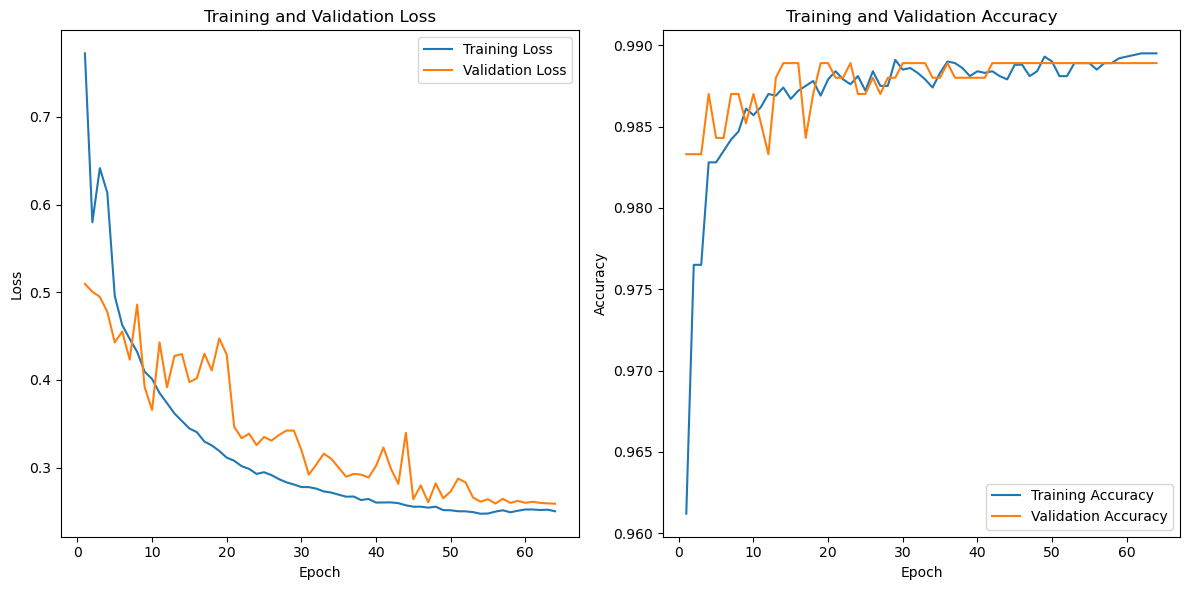
\includegraphics[width = 0.8\textwidth]{resnet_bigure_nmf.png}
  \caption{RNB-NMF各epoch的损失曲线以及准确率曲线}
  \label{fig:ResNet-BiGRU-NoFusion}
\end{figure}

\begin{figure}[htbp]
  \centering
  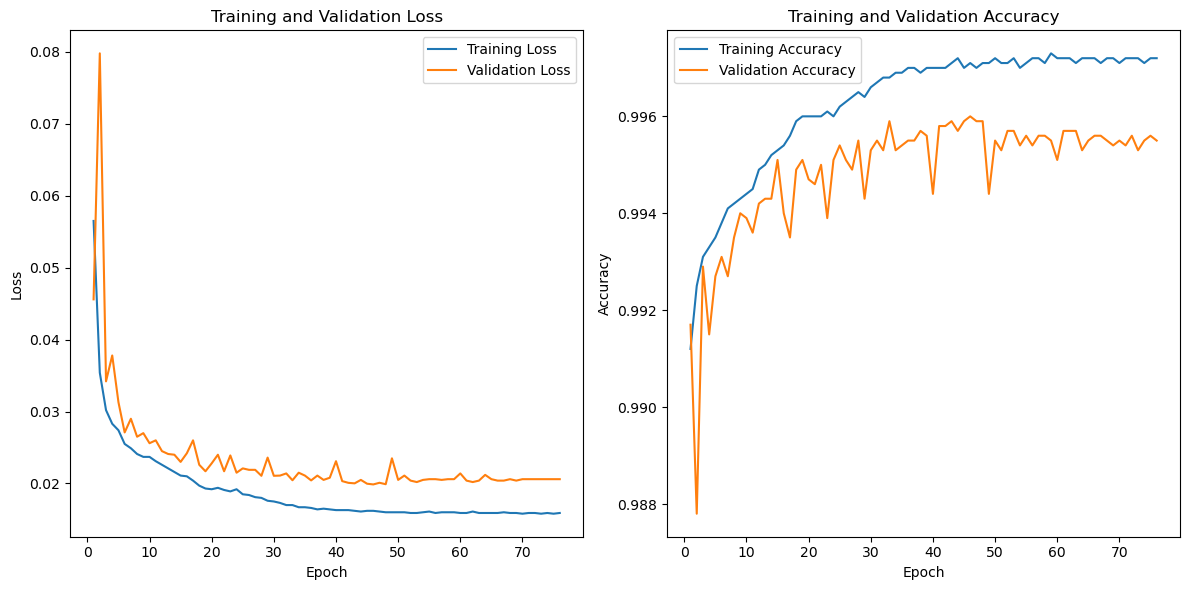
\includegraphics[width = 0.8\textwidth]{resnet_bigure_curve.png}
  \caption{RNB-MF各epoch的损失曲线以及准确率曲线}
  \label{fig:ResNet-BiGRU-Fusion}
\end{figure}
图~\ref{fig:ResNet-BiGRU-NoFusion}~、~\ref{fig:ResNet-BiGRU-Fusion}~分别是未经过模态融合的残差网络和双向门控循环单元的组合以及经过模态融合的残差网络和双向门控循环单元的组合。
通过观察损失函数图表。未经模态融合的模型训练和验证损失都在逐渐减小,但验证损失的波动较大,这可能表明模型在训练集上有过拟合的趋势。
相比之下,经过模态融合的模型损失下降更为平滑,且在训练后期,验证损失几乎与训练损失保持一致,这表明模型具有更好的泛化能力。\par

从准确率图表来看,未经模态融合的模型的准确率虽然相对较高,但在训练过程中出现了一些波动,尤其是验证准确率,这进一步暗示了可能的过拟合问题。
然而,经过模态融合的模型不仅在训练初期准确率快速攀升,而且在后续训练中维持在非常高的水平,几乎没有波动,这显示了模型对于训练和验证数据的稳定预测能力。\par


\section{本章小结}
本章主要围绕RNB-MF模型展开,首先从模型的原理和结构入手,接着详细介绍了模型在数据集上针对性能进行评估的整个过程,包括特征编码、过采样、模型构造、模型训练以及实验结果分析。
通过在实验数据集上与众多经典机器学习和深度学习模型进行对比分析,结果显示我们的模型展现出了显著的优势。\par

然而,在执行多分类任务时,我们观察到,尽管采用了过采样技术,某些攻击类型由于样本数量本身不足,其检测性能仍未显著提高。
为了增强模型对这些少见攻击类型的识别能力,我们可以考虑两种策略:一是通过收集更多的少数类样本来增加数据集中的实际样本量;二是通过调整权重交叉熵损失函数来提高这些特定攻击类型的损失权重。
采用后一策略可能会使模型在提高某一攻击类型的识别率的同时牺牲总体的检测精度,导致误报率升高。
这种权衡需要仔细考虑,在实际应用中需要根据具体情况来平衡检测的敏感性和误报率。
未来的工作可以集中在寻找更有效的数据平衡方法或损失函数,以改善少数类的检测能力,同时保持模型整体的准确性。\par


综上我们可以得出结论,经过模态融合的模型在损失减少和准确率提高方面表现出显著的优势。
模态融合策略有效提高了模型的稳定性和泛化性能,这在处理实际应用中的复杂数据时尤为重要。
通过整合残差网络和双向门控循环单元的特性,模态融合策略可能帮助模型更好地捕获数据的时间依赖性和深层特征,从而提高整体性能。